% latexmk -pvc -pdf
\documentclass[9pt, a4paper]{article}
\usepackage[margin=0.65in]{geometry}
\usepackage{multicol}
\usepackage{amsmath,amsthm,amsfonts,amssymb}
\usepackage[english]{babel}
\usepackage{blindtext}
\usepackage{caption}
\usepackage{graphicx}
\newenvironment{Figure}
    {\par\medskip\noindent\minipage{\linewidth}}
    {\endminipage\par\medskip}

\title{
    
}
\author{Ana C. Fabela Hinojosa
\small{School of Physics and Astronomy, Monash University}}
\date{Submitted: \today}

\begin{document}
\maketitle

\begin{abstract}

\end{abstract}

\section{Introduction}
\begin{multicols}{2}
The least penetrating type of ionizing radiation consists of two protons and two neutrons (nucleons) bound together in alpha particles. These relatively large particles are also known as alpha rays, alpha radiation or helium-4 nuclei\cite{alpha}.

When an atom's nucleus emits an alpha particle, the atom's mass number decreases by four due to the loss of the four nucleons in the alpha particle\cite{alpha}. 




\section{Background Theory}


\subsection{}


\section{Method}
 

\subsection{}


\subsection{Experimental procedure}

\subsection{}


\section{}

\subsection{}



% \begin{Figure}
%  \centering
%  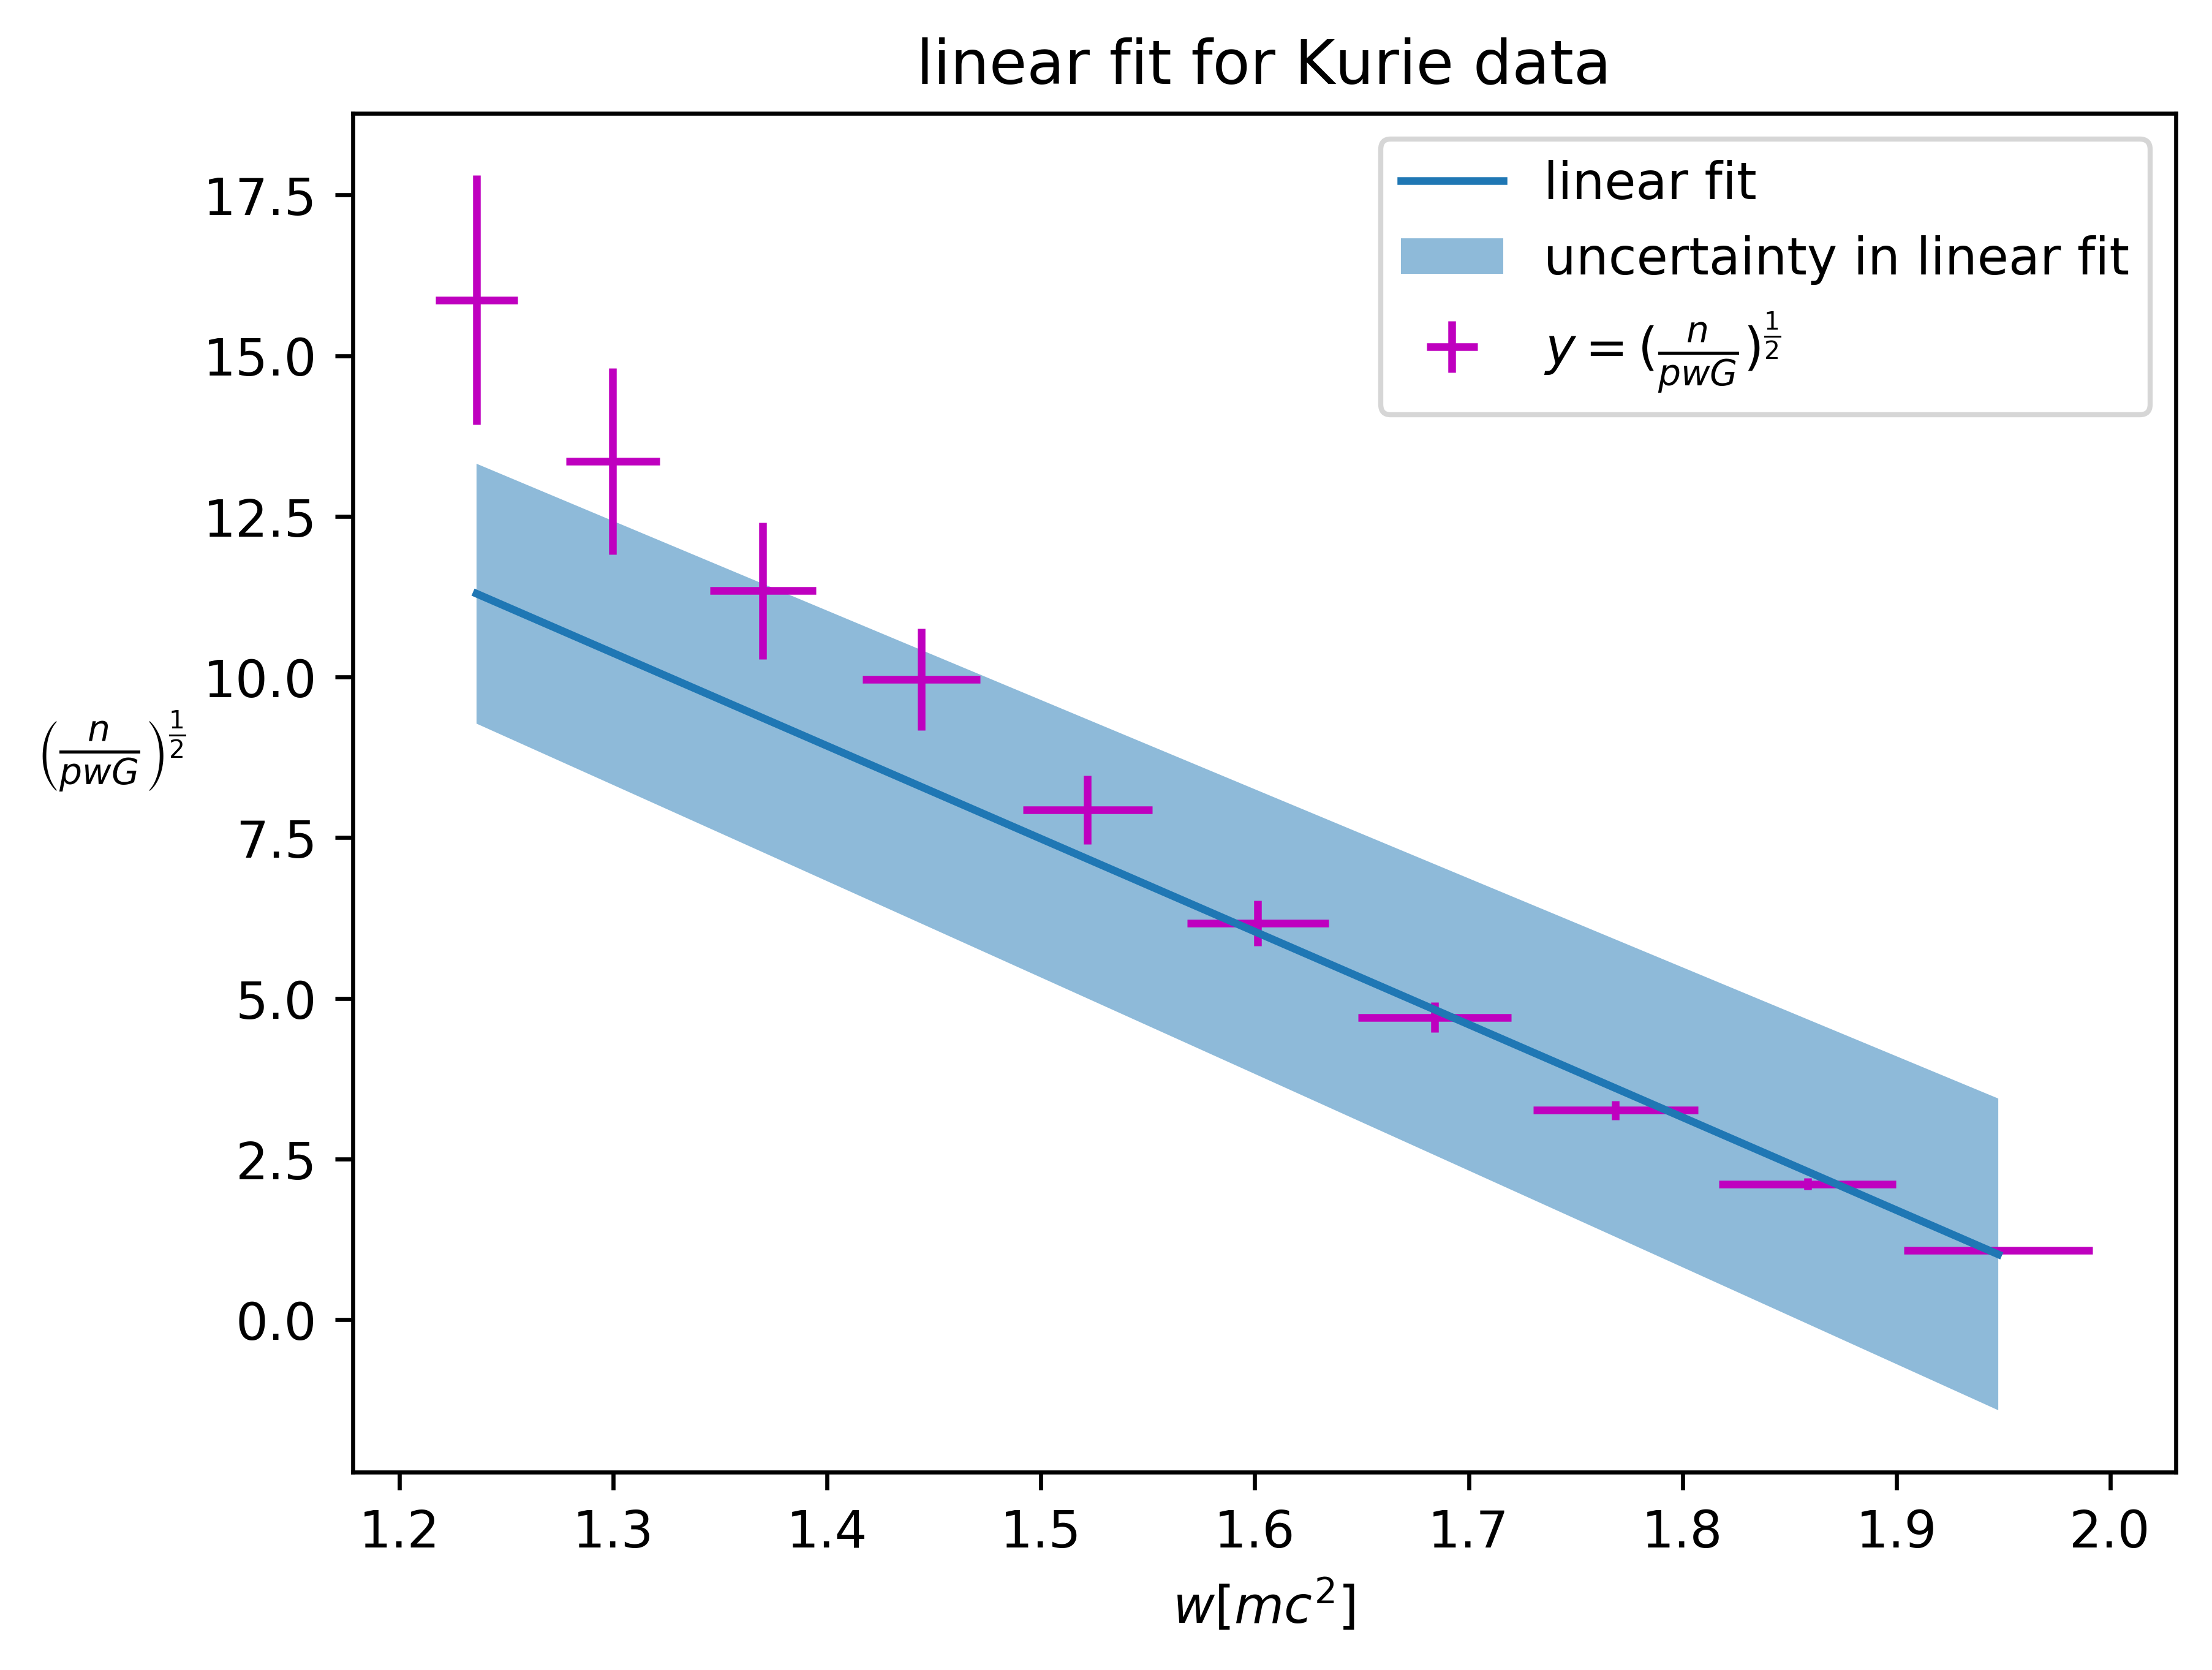
\includegraphics[width=\linewidth]{Kurie_linear_data_plot.png}
%  \captionof{figure}{Linear fit was obtained using the curve\_fit optimisation algorithm from the Scipy library.}
% \end{Figure}

% \begin{Figure}
%  \centering
%  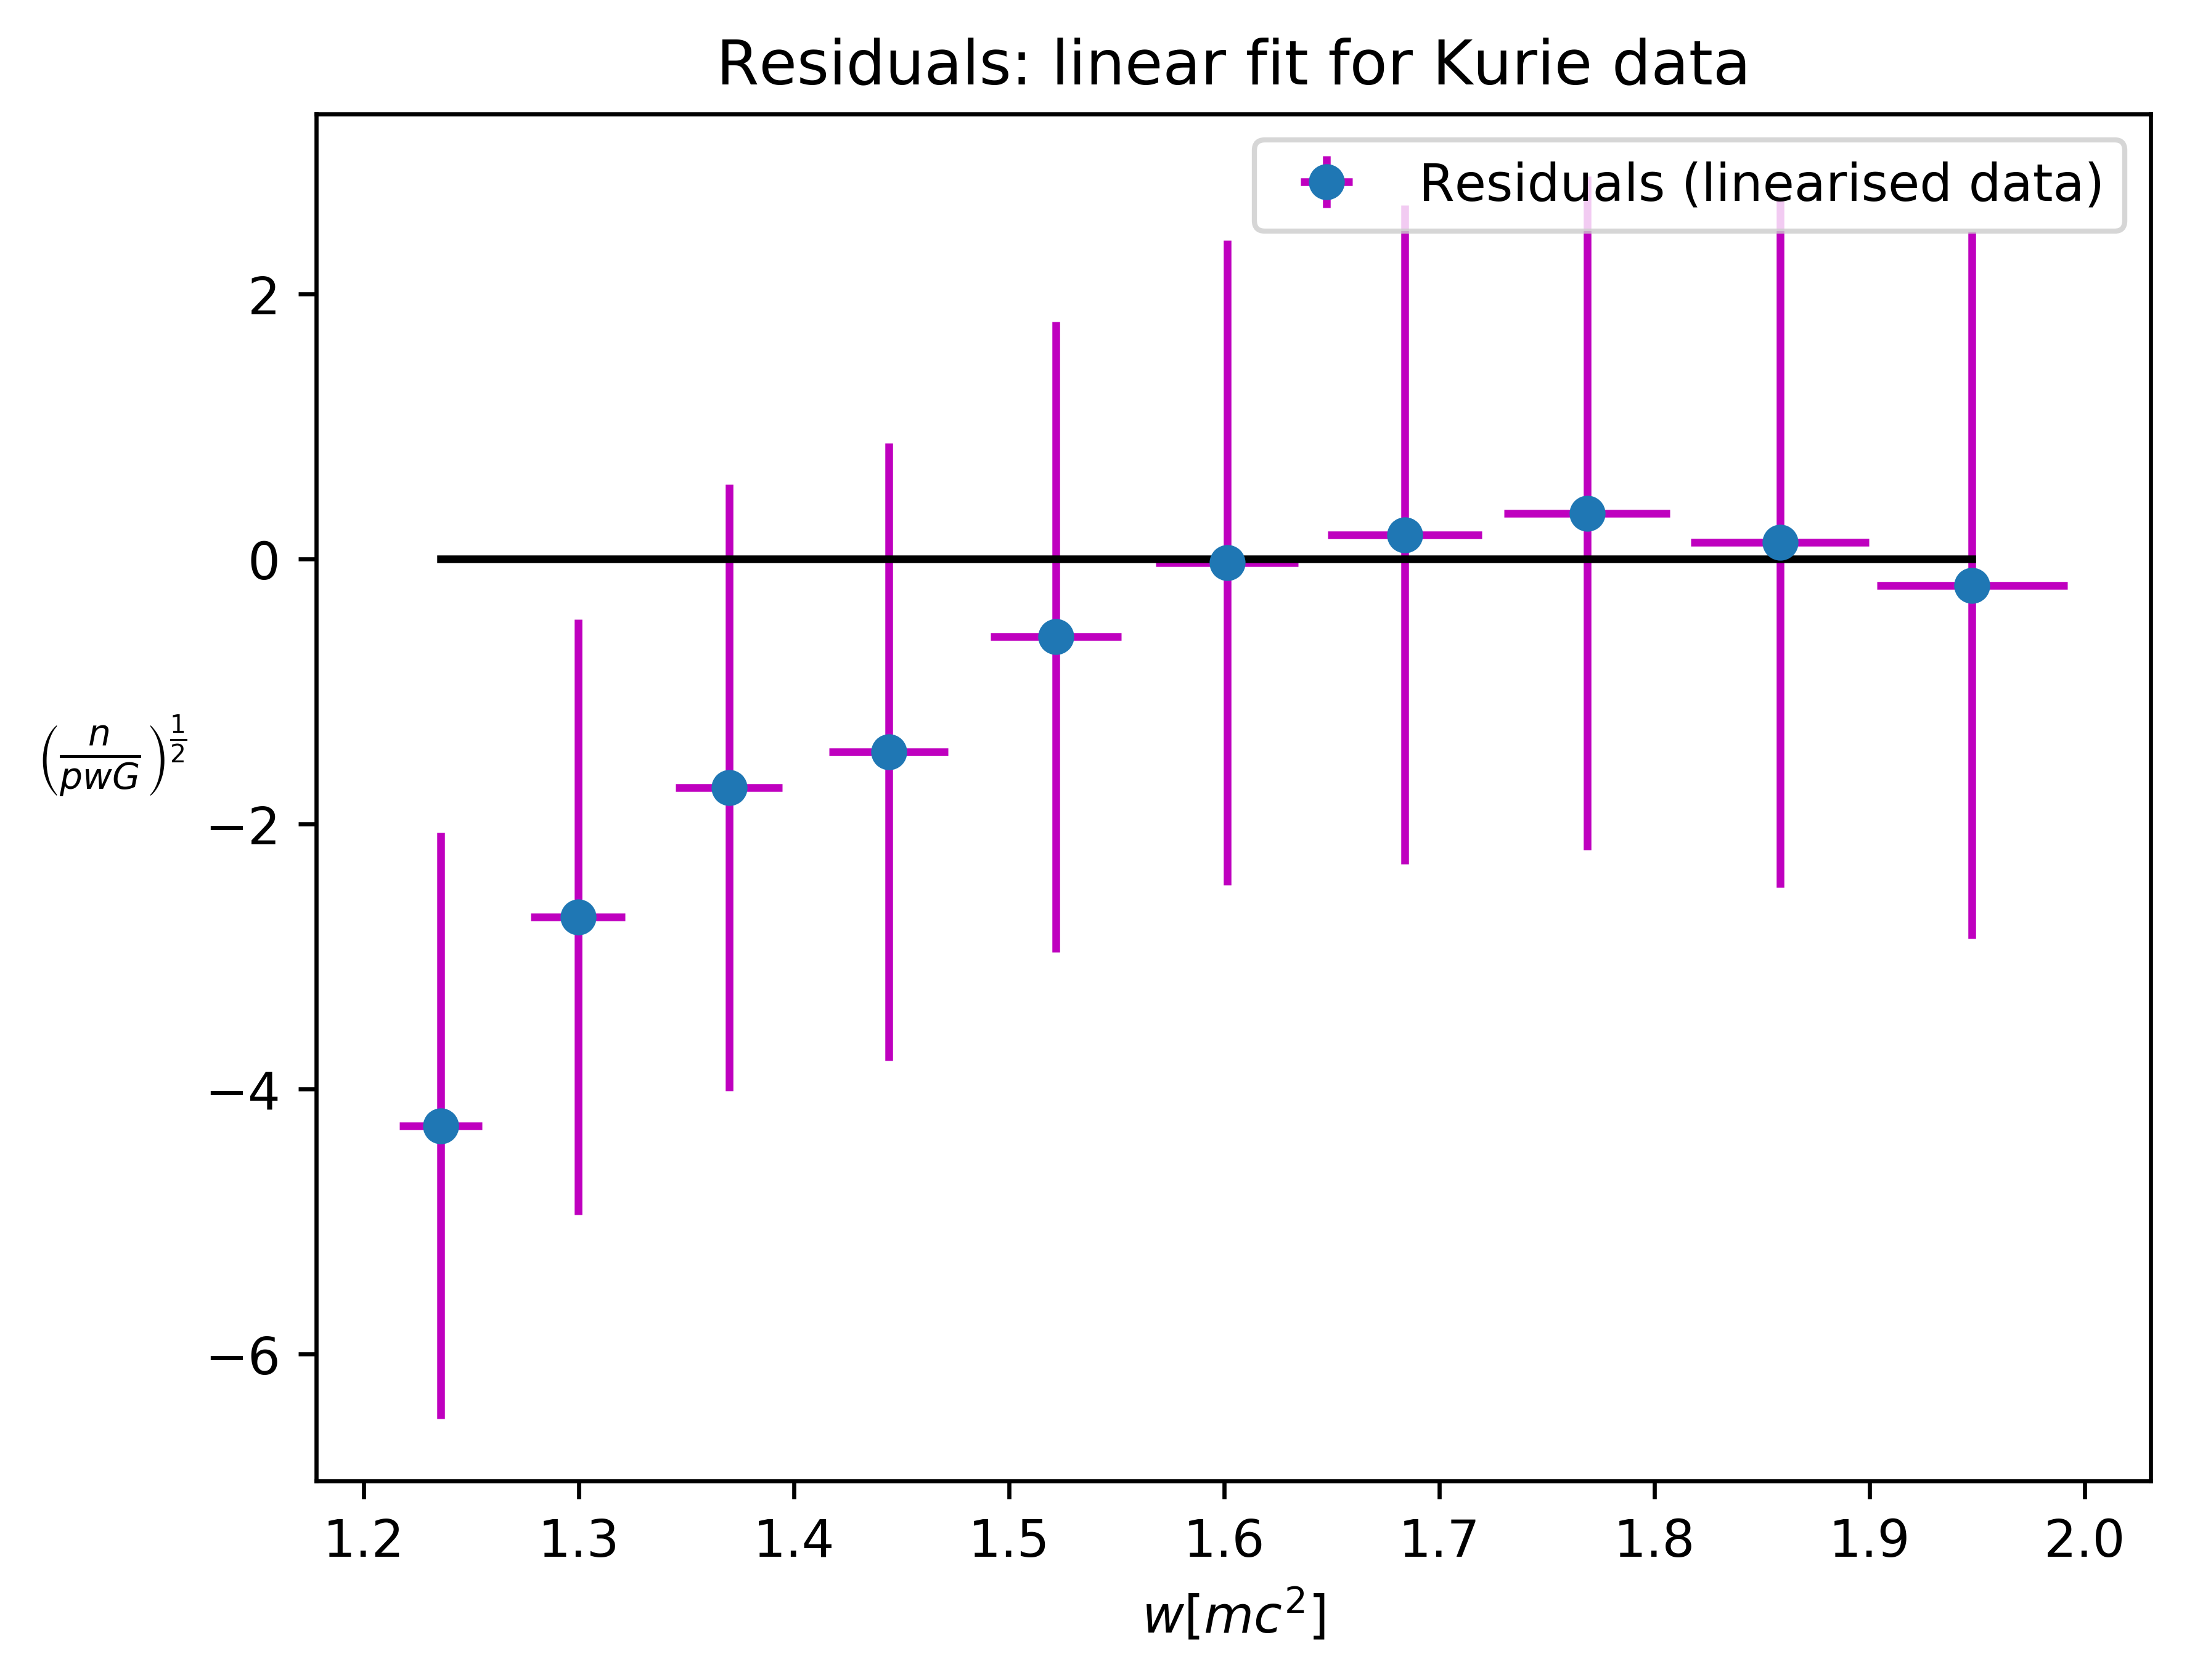
\includegraphics[width=\linewidth]{linear_residuals_Kurie_linear_data.png}
%  \captionof{figure}{Linear fit residuals for optimised Kurie plot data.}
% \end{Figure}


\section{Discussion}



\section{Conclusion}



\end{multicols}
\bibliography{mybib}
\bibliographystyle{unsrt}
\end{document}


% \begin{equation} 
% \end{equation}


% \begin{equation} ,
% \end{equation}
